\documentclass[journal]{IEEEtran}
\usepackage{cite}
\usepackage{amsmath,amssymb,amsfonts}
\usepackage{graphicx}
\usepackage{booktabs}
\usepackage{textcomp}
\usepackage{xcolor}
\usepackage{url}
\graphicspath{{figures/}}
\setlength{\tabcolsep}{3.5pt}

\begin{document}

\title{FidelityMem: Recall-Constrained Adaptive Hybrid Memory\\ for LLM Agents}

\author{Vaibhav~Bansal%
\thanks{V. Bansal is an independent researcher (e-mail: vaibhav.bansal2020@gmail.com). Code, benchmark generator, evaluation stack and all result files are released as the \texttt{fidelitymem} Python package.}}

\markboth{Manuscript, October 2026}{Bansal: FidelityMem}

\maketitle

\begin{abstract}
Long-running LLM agents accumulate far more history than fits in a context window. Memory systems compress, route and retrieve that history, but compression that preserves topic can still delete the entity, number, date or negation a later question needs, and no deployed system exposes evidence recall as a constraint it is required to meet. We present FidelityMem, a memory layer whose control variable is a recall-retention bound: minimise storage, context tokens and latency subject to the compressed index retaining at least $\rho$ of the recall of the best raw retrieval available. The bound is enforced at two points. At admission, a deterministic fidelity gate generates entity, number, date and negation probes from the raw source and backs the compressor off level by level until the compressed form satisfies them. At policy time, a guarded controller measures retention on probe queries, searches over compression level, retrieval depth, expansion budget, route pool, gate profile and dense-route weight, confirms the cheapest feasible configuration on a hold-out split, and keeps the previous policy for rollback. We evaluate on a consistent-world synthetic benchmark at 300 to 10\,000 records and on LoCoMo at session and turn granularity, against eleven baselines including architecture-faithful re-implementations of Mem0, Letta/MemGPT, Zep/Graphiti, A-MEM and HippoRAG that share the same extractors, BM25 and embedder. On the synthetic benchmark FidelityMem reaches the highest Recall@10 and complete-evidence-set recall at every scale while storing 41--48\% of the raw tokens. On LoCoMo, with a sentence embedder, BM25 alone is the strongest retriever (Recall@10 0.914) because the benchmark's questions reuse the evidence's words; the controller detects this from the query log and ties it (0.913), and self-generated probes are shown to be unreliable on chat. When the questions are paraphrased with synonyms, BM25 loses 28 points and lexical--dense fusion 19. Calibrated on each regime's query log alone, the controller selects lexical-only retrieval on literal queries and lexical+dense on paraphrased queries, landing within 0.2--0.7 points of the best fixed configuration in every regime. A Claude reader and judge on 200 LoCoMo questions give 63.0\% accuracy against BM25's 64.5\%, and 61.5\% at 21\% lower cost with an LLM compressor under the gate. We also report what did not work: fixed route weights, a semantic-codebook trie, a hash-map semantic lexicon, query rewriting, LLM reranking, and a leak between a learned embedder and the controller's calibration split.
\end{abstract}

\begin{IEEEkeywords}
Agent memory, retrieval-augmented generation, hybrid retrieval, lossy compression, reciprocal-rank fusion, recall constraint, constrained optimisation, LLM agents.
\end{IEEEkeywords}

\IEEEpeerreviewmaketitle

\section{Introduction}
\IEEEPARstart{A}{gent} memory research has converged on a shared architecture: a short working context, typed long-term stores, compression, and retrieval that fuses lexical, dense and graph signals. MemGPT introduced hierarchical context management \cite{memgpt}; HippoRAG added entity graphs and personalised PageRank \cite{hipporag}; Zep/Graphiti added a bi-temporal knowledge graph \cite{zep}; Mem0 reduced memory to atomic LLM-extracted facts \cite{mem0}; A-MEM linked notes by similarity \cite{amem}; and 2026 work (EvolveMem, MemRL, Agent Zero Memory, LazyMem, CrystalMem, ARC, MemRefine) refines routing, consolidation, learned utility and compaction \cite{evolvemem,memrl,agentzero,lazymem,crystalmem,arc,memrefine}. The components are no longer novel individually.

What remains unsolved is \emph{control}. Every system above decides how much to compress and how deep to retrieve with fixed heuristics or with learning aimed at answer accuracy. None states a recall bound and enforces it. The consequence, documented in recent fidelity studies, is silent evidence loss: a $36.7\times$ compression of structured facts left 60\% irrecoverable \cite{facts}; summarisers keep type hints and drop the qualifier ``everywhere'' \cite{fidelity}; rewrites launder hedged hearsay into asserted fact \cite{factwash}. Retrieval metrics do not catch this because the right memory id is retrieved while the fact inside it is gone.

A second unsolved problem is the choice of retrieval regime. Hybrid retrieval is the default in every system above, with fixed or per-query fusion weights \cite{tfusion,wrrf,vstash}. Our measurements show that the right regime depends on how questions are phrased relative to the evidence: on LoCoMo, where annotators reused the evidence's words, BM25 beats every hybrid; once questions are paraphrased, the ordering reverses. A 2026 study found no lightweight adaptive router that beat a fixed sparse--dense blend under cross-validation \cite{fairness}.

FidelityMem's contribution is therefore not a new store but a recall-constrained controller with an enforceable gate, and a protocol that can measure whether the bound holds. Our claims are deliberately narrow:
\begin{enumerate}
\item A deterministic fidelity gate, built from the raw source, prevents fact loss at admission without an LLM and with no labels (Sec.~\ref{sec:gate}).
\item A guarded search over discrete compression levels, depths, expansion budgets, route pools, gate profiles and dense-route weights finds the cheapest policy that holds a retention bound $\rho$ and confirms it out of sample (Sec.~\ref{sec:controller}).
\item Relation chaining after fusion recovers the second hop of two-hop questions that reciprocal-rank fusion buries (Sec.~\ref{sec:retrieval}, Sec.~\ref{sec:ablation}).
\item Under a fixed protocol with shared components, this design dominates six current memory architectures on recall, complete-set recall, stored tokens and tokens per query at every synthetic scale tested (Sec.~\ref{sec:synthetic}). On LoCoMo it ties the strongest baseline, BM25, and does not beat it; we show why (Sec.~\ref{sec:paraphrase}).
\item The controller selects the retrieval regime from the query log alone, lexical-only when queries are literal and lexical+dense when they are paraphrased, matching the best fixed configuration in each regime out of sample (Sec.~\ref{sec:regime}).
\item Self-generated probes, which suffice on fact-dense text, are unreliable on conversational data; a query log is required (Sec.~\ref{sec:minilm}).
\end{enumerate}

\section{Related Work}
Table~\ref{tab:related} places FidelityMem against the nearest work on three axes: memory architectures, compression fidelity, and adaptive hybrid retrieval. Two results frame our retrieval findings. Ref.~\cite{tfusion} reports lexical--dense fusion beating BM25 in every LoCoMo category; we find fusion one point below BM25 at session granularity with a MiniLM embedder, and attribute the difference to retrieval unit and embedder, which Sec.~\ref{sec:paraphrase} tests directly by paraphrasing the questions. Ref.~\cite{fairness} reports that oracle tuning of the sparse--dense weight on financial documents has 22\% headroom which no lightweight adaptive router realised under cross-validation; Sec.~\ref{sec:regime} shows a selector that does realise it, a discrete guarded search with an out-of-sample confirmation step rather than a per-query predictor. Benchmarks: LoCoMo \cite{locomo} provides evidence dialogue ids per question, which we use as exact retrieval ground truth; LongMemEval \cite{longmemeval}, MemBench \cite{membench} and DolphinBench \cite{dolphin} are the other standard suites.

\begin{table*}[t]
\caption{Nearest work and the difference}
\label{tab:related}
\centering
\footnotesize
\begin{tabular}{p{3.0cm}p{4.3cm}p{3.6cm}p{5.8cm}}
\toprule
System & Core mechanism & FidelityMem takes & FidelityMem adds \\
\midrule
MemGPT / Letta \cite{memgpt} & Core + recall + archival tiers, agent-driven paging & Working vs long-term split & Retention-scored window with boundary triggers; no agent in the loop \\
HippoRAG \cite{hipporag} & OpenIE entity graph, PPR seeded by query entities & Graph seeded by query entities, retrieve-then-expand & Relation-following with hub penalty; relation chaining after fusion \\
Zep / Graphiti \cite{zep} & Bi-temporal entity graph, hybrid search, edge invalidation & Temporal validity, supersede-not-delete & Contradiction limited to exclusive predicates; fidelity gate \\
Mem0 \cite{mem0} & LLM-extracted atomic facts, vector search, add/update/delete & Fact-level dedupe & Raw evidence retained and expandable; no LLM needed to ingest \\
A-MEM \cite{amem} & Notes with keywords, links to neighbours & Linked expansion & Explicit relations instead of similarity links \\
R$^3$Mem \cite{r3mem} & Reversible compression via virtual memory tokens & Reversibility as a requirement & Reversibility by immutable raw pointer rather than model inversion \\
EvolveMem \cite{evolvemem}, MemRL \cite{memrl} & Learned retrieval configuration / utility & Feedback-driven utility & Constraint-based rather than accuracy-based optimisation, hold-out gate, rollback \\
Agent Zero Memory \cite{agentzero} & Parallel stores, provenance, citation-locked answers & Provenance on every memory & Admission-time gate rather than answer-time verification \\
LazyMem \cite{lazymem} & Retrieve broadly, construct context selectively & Query-time expansion & Expansion triggered by confidence, exact-value need and conflict \\
CrystalMem \cite{crystalmem} & Four fidelity states under a byte budget; gate on promotion & Fidelity as an explicit state & Budget-driven demotion; FidelityMem's bound is on measured recall, not bytes \\
ARC \cite{arc} & Older observations replaced by addressable citations & Raw source always addressable & Compaction is unconditional; FidelityMem compresses only when the gate certifies it \\
MemRefine \cite{memrefine}, rate--distortion view \cite{ratedist} & Compression under a hard budget; compaction as rate--distortion & The budget/fidelity trade-off as the object of study & Recall floor instead of a budget; out-of-sample confirmation \\
Lexical--dense fusion \cite{tfusion}; adaptive WRRF \cite{wrrf}; vstash \cite{vstash} & Hybrid retrieval for agent memory with fixed or per-query fusion weights & Weighted RRF over lexical and dense routes & Weight chosen by the controller from the query log under the recall bound, together with the compression level, confirmed on a hold-out split \\
Facts as objects \cite{facts}, Fidelity before structure \cite{fidelity}, FACTWASH \cite{factwash} & Evidence that gist compression loses facts, qualifiers and attribution & Motivation and probe design & A gate that enforces it per memory \\
\bottomrule
\end{tabular}
\end{table*}

\section{System Design}
\begin{figure*}[t]
\centering
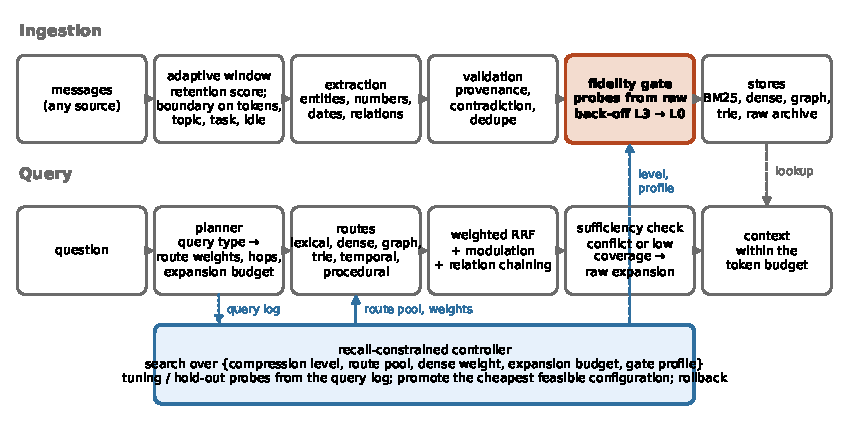
\includegraphics[width=\textwidth]{fig_architecture.pdf}
\caption{FidelityMem workflow. Top: ingestion through the adaptive window, extraction, validation and the fidelity gate into the stores. Bottom: a query through the planner, the routes, weighted RRF with modulation and relation chaining, the sufficiency check and the token budget. The controller sets the route pool and weights on the query side and the compression level and gate profile on the ingestion side, from the query log.}
\label{fig:arch}
\end{figure*}

\subsection{Data model}
An \emph{episode} is immutable raw text with provenance (source id, type, tenant, namespace, timestamp, trust, authority). A \emph{memory} is a derived, searchable record pointing at exactly one episode: compressed text, compression level, extracted entities, numbers, dates, negated sentences, relations, types (semantic, episodic, procedural, relational), confidence, validity interval, utility and a fidelity score. Memories are superseded, never deleted; user-requested forgetting removes both memory and episode.

\subsection{Adaptive working window and admission}
Each message carries a retention score $R(m) = w_s S_{\mathrm{sem}} + w_r S_{\mathrm{rec}} + w_i S_{\mathrm{imp}} + w_t S_{\mathrm{task}} + w_c S_{\mathrm{conf}} + w_u S_{\mathrm{util}}$, with task continuity weighted highest (0.30) so that an unresolved task is evicted last. Boundaries fire on token pressure, topic shift (low similarity to the running topic vector and no shared entities), task completion and inactivity; each boundary hands its segment to extraction. Admission runs three validation stages. Stage 1 attaches provenance, detects contradictions (polarity flip on a near-identical statement, conflicting values for the same entity set, or a conflicting object for an \emph{exclusive} predicate such as ``runs on''), supersedes the older memory when the new source is trusted, and demotes any instruction found in untrusted content from procedural to episodic. Stage 2 scores durability from importance, fact density and length and drops near-duplicates, where a duplicate requires identical entity, number and date sets as well as high token overlap. Stage 3 is the fidelity gate.

\subsection{Reversible compression and the fidelity gate}
\label{sec:gate}
Compression is a four-level ladder: L0 raw; L1 extractive at about 60\% of sentences by salience (centrality, fact count, negation, lead bias); L2 key facts, keeping only sentences that carry an entity, number, date or negation; L3 gist, a single salient sentence. An LLM compressor plugs in through a one-method protocol and is gated identically.

From the \emph{raw} text we build a probe set: one probe per entity (weight 1), number (1.5), date (1.5) and negated sentence (2; satisfied only if at least 60\% of its content words and a negation cue survive). Two profiles exist: \emph{facts}, as above, and \emph{content}, which adds up to 16 salient content-word probes at weight 0.5 and is therefore stricter on conversational text. The gate accepts a compressed form at level $\ell$ iff its weighted probe score is at least $\rho$; otherwise it backs off to $\ell-1$, and L0 always passes. Because probes are generated from the source rather than the summary, the gate measures what was lost. The probe set is stored with the memory so that recompression under a new policy reuses it.

\subsection{Query-aware hybrid retrieval}
\label{sec:retrieval}
The planner classifies a query as factual, temporal, multi-hop, exact, procedural or code-review and sets route weights, graph hops, expansion budget and whether raw expansion is mandatory. The controller's route pool is authoritative: the planner may weight routes but never adds one the controller excluded. Routes: BM25 ($k_1 = 1.5$, $b = 0.75$); dense (any embedder through one protocol: a hashing embedder for hermetic tests, spaCy word vectors, or MiniLM-L6 over overlapping 120-word windows averaged and renormalised); a relation graph with relation-following before co-mention, a hub penalty $1/(1 + \log(1 + \mathrm{degree} - 3))$ and no traversal through hub entities above degree 40, seeded from query entities and from relation objects of the top-3 BM25 hits, with a bridged second pass that re-issues the query anchored on each bridge entity; a trie over identifier-like tokens and 2--4-gram phrases; a temporal route (episodic memories by lexical match, recency-ordered only when the query asks for recent state); and a procedural route. An optional semantic-codebook trie route and a semantic lexicon for BM25 query expansion are described with their results in Sec.~\ref{sec:routeweights} and Sec.~\ref{sec:semtrie}.

Route results are fused by weighted reciprocal-rank fusion, $s(d) = \sum_r w_r/(60 + \mathrm{rank}_r(d))$, and multiplied by $1 + 0.05\,\mathrm{recency} + 0.2\tanh(\mathrm{utility}) + 0.05\,\mathrm{authority}\cdot\mathrm{confidence} + \mathrm{type\ boost}$. The factor is multiplicative and small because RRF differences between adjacent ranks are about 1.6\%, so additive bonuses would dominate the ordering. Two steps follow that the baselines lack. \emph{Relation chaining}: if a top result states $A \xrightarrow{p} B$ with $A$ named in the query, the memories in which $B$ is a relation subject are promoted to just below it; this recovers the second hop that RRF ($k = 60$) otherwise buries under weakly matched filler. \emph{Sufficiency and expansion}: a memory is expanded to its raw episode, within a budget, when the task is exact, confidence or fidelity is low, retrieved memories conflict on an exclusive predicate, the query's content words are barely covered by the compressed text, or a multi-hop query hits a memory without relations. A conflict counts as unresolved only while a party to it is compressed and unexpanded. Context is then trimmed to the token budget, falling back from raw to compressed before dropping.

\subsection{Recall-constrained controller}
\label{sec:controller}
\begin{figure}[t]
\centering
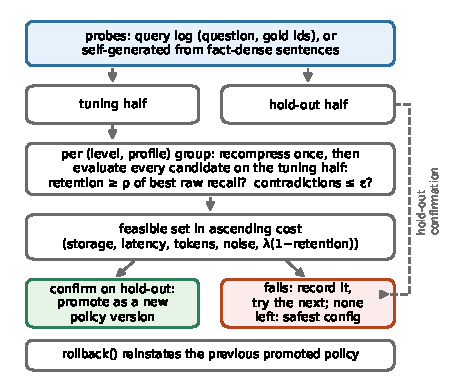
\includegraphics[width=\columnwidth]{fig_controller.pdf}
\caption{The controller's guarded search. Candidates are evaluated on the tuning half, walked in ascending cost, and promoted only after confirming on the hold-out half; a failed candidate is recorded and never retried.}
\label{fig:ctrl}
\end{figure}
Let $\pi$ be a configuration: compression level in $\{0,1,2,3\}$, top-$k$ in $\{5,10\}$, expansion budget in $\{0,2\}$, one of five route pools from \{lexical\} to all six routes, gate profile in \{facts, content\}, and dense-route weight in $\{0.5, 1.0\}$ (ignored when the dense route is not in the pool). The controller minimises
\begin{equation}
\begin{split}
\mathrm{cost}(\pi) = \; & \alpha\,\mathrm{StorageRatio} + \beta\,\mathrm{Latency} + \gamma\,\mathrm{TokensPerQuery} \\
& + \delta\,\mathrm{Noise} + \lambda\,\bigl(1 - \mathrm{Retention}(\pi)\bigr)
\end{split}
\label{eq:cost}
\end{equation}
subject to $\mathrm{Retention}(\pi) = \mathrm{Recall}_\pi@K / \mathrm{Recall}_{\mathrm{rawbest}}@K \ge \rho$ and $\mathrm{UnresolvedContradictionRate} \le \varepsilon$. The reference $\mathrm{Recall}_{\mathrm{rawbest}}$ is the best uncompressed retrieval over all route pools, not the candidate's own L0 twin; without this the constraint is vacuous for a candidate whose route pool is itself weak. The $\lambda$ term charges recall lost inside the bound so that two feasible candidates are not ordered by cost alone.

Retention cannot be observed on live queries, so it is measured on probe queries (Fig.~\ref{fig:ctrl}). Self-generated probes take, for a sampled episode, its most fact-dense sentence (an entity plus a value or a second entity) with a third of its words dropped; the probe must retrieve that episode. A query log supplies (question, gold episode ids) pairs instead. Probes are split into tuning and hold-out halves. Every candidate is evaluated on the tuning half, grouped by level and profile so the store is recompressed once per group, and only memories whose text changes are re-indexed. Feasible candidates are walked in ascending cost and confirmed on the hold-out half; the first that confirms is promoted as a new policy version. A candidate that fails confirmation is recorded and not retried. If none confirms, the safest configuration (raw, widest pool) is promoted. Rollback reinstates the previous promoted policy.

\subsection{LLM components}
A Claude-backed compressor, extractor, reader, judge, query rewriter and reranker are implemented behind the same protocols as the deterministic components, with a mock for tests. The compressor and extractor are gated and controlled exactly as the extractive ones; the reader and judge are used only for evaluation.

\section{Experimental Protocol}
\textbf{Synthetic dataset.} A single seeded generator produces a consistent world: 200 services, each with one database, one owner and one dependency, so no gold fact is legitimately contradicted. Every episode is a fact sentence embedded in 2--4 sentences of realistic workplace filler, so compression has something to lose. Question families, in rotation: factual (``where does X store session data''), temporal (``when did the migration of X fail''), multi-hop (``which database does the service that X depends on run on'', two gold episodes), exact (``what is the exact connection pool cap for X'', two numbers and a negated constraint). Distractors fill to the record count: 30\% hard (same service and database names, no decision) and 70\% off-topic; 2\% are procedural rules. Record levels 300, 1\,000, 3\,000 and 10\,000 with 200 questions each.

\textbf{Real data.} LoCoMo \cite{locomo}: 10 multi-session conversations, 5\,882 turns, 1\,986 questions with evidence dialogue ids as retrieval ground truth; categories multi-hop, temporal, open-domain, single-hop and adversarial (no gold evidence, excluded from recall). Two granularities: one memory per turn (hard retrieval, little to compress) and one per session (272 sessions, the realistic compression target). Per seed, 30\% of questions are held out as the controller's query log and never scored; the controller runs twice, once on self-generated probes and once on that log.

\textbf{Paraphrase regimes.} Every LoCoMo question is rewritten with WordNet synonyms: for each eligible content word (alphabetic, longer than three characters, not a stop word, not an entity, date or number, not sentence-internal capitalised) the first lemma of a different stem among its synsets replaces it with probability $r$. At $r = 0.5$, 1\,615 of 1\,982 questions change and 45\% of eligible words are replaced; at $r = 1.0$, 1\,933 change and 91\% are replaced.

\textbf{Metrics.} Recall@$K$ against gold episode ids, complete-evidence-set recall (all gold ids in the top $K$), MRR, nDCG@$K$, tokens per query, p50/p95 retrieval latency, stored tokens, raw-expansion rate, and recall retention against the best raw retrieval. Every multi-seed experiment reports the mean over seeds 0, 1, 2 (synthetic: different worlds; real: different ingestion orders and calibration splits) with a 95\% $t$-interval; single-seed runs report a bootstrap interval over questions. For LLM-judged accuracy we also report abstention rate, context tokens and API cost at list prices.

\textbf{Baselines.} Classic: fixed sliding window, BM25, dense, BM25+dense RRF, lossy summary (L3 gist without a gate) + BM25. Architecture-faithful re-implementations, each using the same extractors, BM25 and embedder as FidelityMem: \emph{window+trie} (last-50 window plus trie exact/prefix index); \emph{MemGPT-style} (core recent block always in context + vector recall/archival); \emph{Mem0-style} (every entity-bearing sentence is an atomic memory, deduped, vector-only, mapped back to its episode); \emph{Zep-style} (entity graph with relations + BM25 + dense, RRF, 1-hop expansion); \emph{A-MEM-style} (each note linked to its 3 nearest neighbours at insert; retrieve then follow links); \emph{HippoRAG-style} (entity graph seeded by query entities, 2-hop spreading, fused with dense at weight 1.5). These are not vendor code: the vendors require an LLM to ingest, which would confound architecture with model.

\textbf{Embedders.} All dense routes in every system share one embedder per experiment: spaCy \texttt{en\_core\_web\_md} word vectors (300-d, IDF-weighted mean pooling) in the original runs; all-MiniLM-L6-v2 exported to ONNX and run on CPU, long records embedded as the mean of overlapping 120-word windows, in the runs of Sec.~\ref{sec:minilm} onward; a retrieval-adapted embedder trained per seed in Sec.~\ref{sec:adapted}.

\textbf{LLM evaluation.} A Claude Opus 5.5 reader at low effort answers from the served context only and abstains when the context lacks the answer; a Claude Sonnet 5.5 judge marks the answer against the gold. Claude Haiku 5.5 serves as rewriter and reranker where tested. Test questions are a fixed 200-question sample of the 70\% test split, seed 0.

\textbf{Controls.} Same episodes, questions, seed, $K$, embedder and token accounting for every system; stochastic components are seeded; the controller never sees scored questions; a learned embedder never trains on questions the controller calibrates on (Sec.~\ref{sec:adapted} explains why).

\section{Synthetic Benchmark at Four Scales}
\label{sec:synthetic}
\begin{figure}[t]
\centering
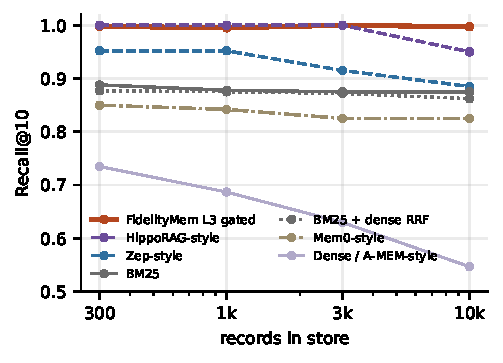
\includegraphics[width=\columnwidth]{fig_scale.pdf}
\caption{Recall@10 against store size (3 seeds). FidelityMem at level 3 holds 0.995--1.000 while storing 44\% of the raw tokens; graph-first architectures fall at 10\,000 records; BM25 never reaches the second hop.}
\label{fig:scale}
\end{figure}
FidelityMem holds 0.995--1.000 Recall@10 and complete-set recall from 300 to 10\,000 records while storing 41--48\% of the raw tokens (Fig.~\ref{fig:scale}, Table~\ref{tab:synthetic}). The HippoRAG-style graph ties it at 300--3\,000 records at full storage and lower nDCG, and falls to $0.950 \pm 0.066$ at 10\,000, where hub entities dilute two-hop spreading; Zep-style falls from 0.952 to 0.885; BM25 stays at 0.875--0.888 and never reaches the second hop (complete-set recall 0.75 at every scale); Mem0-style sits at 0.83 with the smallest index of the baselines (23\% of raw). At 10\,000 records FidelityMem is alone at the top on both recall and complete-set recall.

\begin{table}[t]
\caption{Recall@10 by record count ($K=10$, 3 seeds, word-vector embedder)}
\label{tab:synthetic}
\centering
\scriptsize
\resizebox{\columnwidth}{!}{%
\begin{tabular}{lrrrrr}
\toprule
System & 300 & 1\,000 & 3\,000 & 10\,000 & Storage \\
\midrule
Fixed window & 0.038 & 0.005 & 0.012 & 0.002 & 100\% \\
BM25 & 0.888 & 0.878 & 0.875 & 0.875 & 100\% \\
Dense & 0.735 & 0.687 & 0.630 & 0.547 & 100\% \\
BM25 + dense RRF & 0.877 & 0.875 & 0.872 & 0.862 & 100\% \\
Lossy L3 summary + BM25 & 0.855 & 0.853 & 0.850 & 0.857 & 27\% \\
Window + trie & 0.875 & 0.875 & 0.875 & 0.875 & 100\% \\
MemGPT-style & 0.705 & 0.658 & 0.605 & 0.528 & 100\% \\
Mem0-style & 0.850 & 0.842 & 0.825 & 0.825 & 23\% \\
Zep-style & 0.952 & 0.952 & 0.915 & 0.885 & 100\% \\
A-MEM-style & 0.735 & 0.687 & 0.630 & 0.547 & 100\% \\
HippoRAG-style & 1.000 & 1.000 & 1.000 & 0.950 & 100\% \\
FidelityMem raw (L0) & 0.998 & 0.995 & 1.000 & 0.997 & 100\% \\
FidelityMem L1 gated & 0.998 & 0.995 & 1.000 & 1.000 & 69\% \\
FidelityMem L2 gated & 0.998 & 0.995 & 1.000 & 0.997 & 48\% \\
FidelityMem L3 gated & 0.998 & 0.995 & 1.000 & 0.997 & 44\% \\
FidelityMem controller & 0.998 & 0.995 & 0.977 & 0.997 & 41--48\% \\
\bottomrule
\end{tabular}}
\end{table}

\textbf{Compression without loss.} Levels 2 and 3 store 42--48\% of the raw tokens and serve about 60\% of the context tokens per query with retention 1.0 against L0; the gate backed off on roughly one in six episodes, which is exactly the set where a gist would have dropped a fact. The lossy summary baseline stores less (about 27\%) and loses 2--4 points of recall with wide variance across seeds.

\textbf{Controller choice.} With no access to the questions, the controller selected level 3 (one seed level 1) with the facts gate profile and the two cheapest routes at every scale, and its measured retention is 0.98--1.00. Its latency is the lowest of the FidelityMem rows because it dropped the graph and temporal routes it found unnecessary for the probe distribution; at 3\,000 records one seed's cheaper route set cost multi-hop recall ($0.977 \pm 0.063$), still above the bound.

\textbf{Window + trie.} Perfect MRR on exact-value questions and competitive recall at small scale, but capped at the BM25 ceiling on factual and temporal questions and unable to reach a second hop. This is why the trie is kept as a route inside FidelityMem rather than as the system.

\textbf{Pareto frontier.} On the storage--recall plane at 3\,000 and 10\,000 records (Fig.~\ref{fig:pareto}), the FidelityMem gated levels and the controller form the frontier: no baseline reaches their recall at any storage, and the only baselines with smaller indices (Mem0-style, lossy summary) are 15--17 points below in recall.

\begin{figure}[t]
\centering
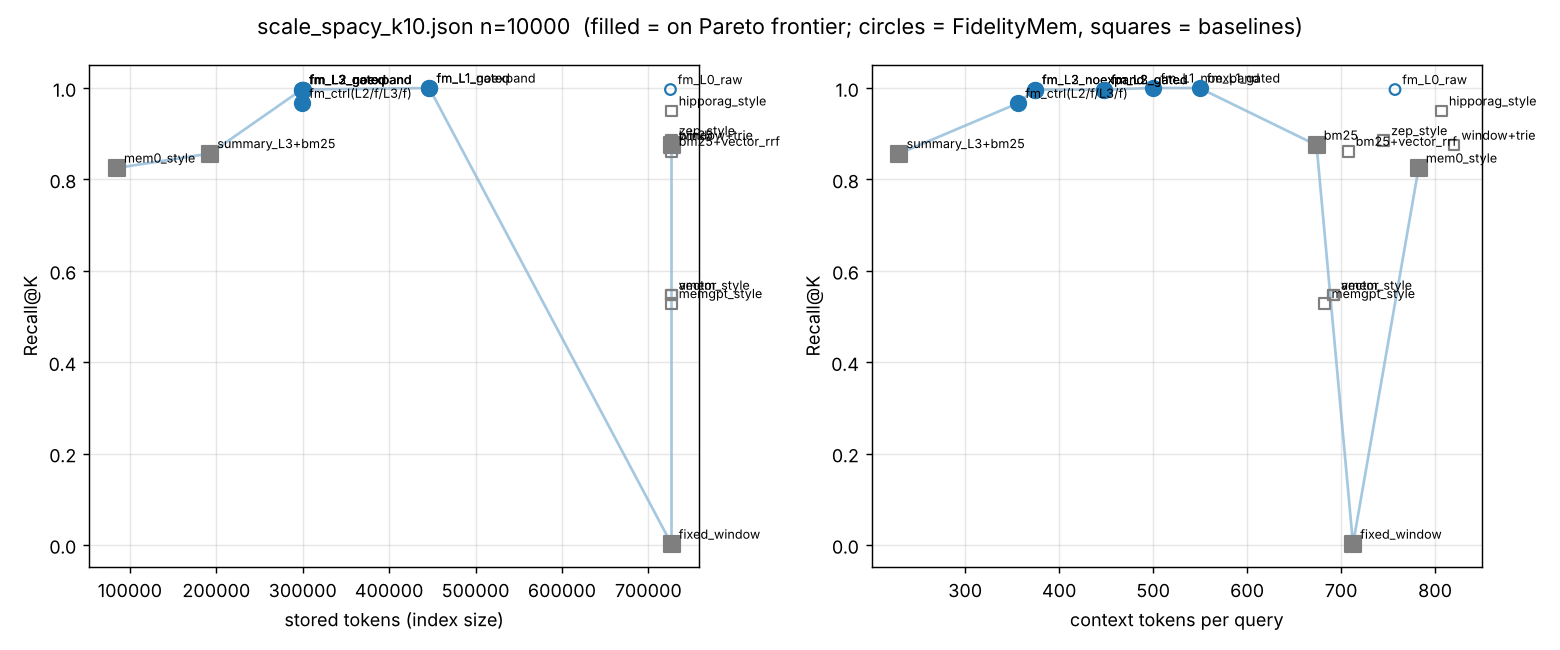
\includegraphics[width=\columnwidth]{pareto_synthetic_10k.png}
\caption{Storage--recall Pareto frontier at 10\,000 records. FidelityMem's gated levels and controller form the frontier; graph-first and atomic-fact architectures are dominated.}
\label{fig:pareto}
\end{figure}

\section{Real Conversation Data: LoCoMo}
\subsection{Session granularity with word vectors ($K=5$, 3 seeds)}
Lexical retrieval is the strongest single signal on human conversation: BM25 alone reaches $0.858 \pm 0.009$ Recall@5 (Table~\ref{tab:locomo5}). Every architecture that fuses a dense or graph signal at equal weight lands well below it, because the word-vector dense route is weak (0.287) and rank fusion lets it outvote BM25's first place. The controller is what makes the architecture safe: with retention measured against the best raw retrieval it drops the dense route on every seed and lands at $0.851 \pm 0.015$ (self-probes) and $0.849 \pm 0.014$ (query log). Compression at $\rho = 0.95$ is small on chat: the facts profile compresses to 22--65\% of raw and retains only 0.79--0.94 of recall, the content profile retains 1.00 and stores 98\%, so the controller keeps near-raw storage. The gate still earns its place: at every level the gated variant beats the ungated one (0.444 vs 0.358 at level 3, facts profile) and needs a quarter of the raw expansions. At turn granularity (5\,880 turns, $K=10$) the ordering is the same with every number lower: BM25 $0.558 \pm 0.014$, the controller $0.534 \pm 0.064$ (self-probes) and $0.529 \pm 0.073$ (query log), Zep-style 0.499, window+trie 0.371, every other architecture 0.13--0.22.

\begin{table}[t]
\caption{LoCoMo sessions, Recall@5, word-vector embedder, 3 seeds. Categories: multi-hop / temporal / single-hop / open-domain}
\label{tab:locomo5}
\centering
\scriptsize
\resizebox{\columnwidth}{!}{%
\begin{tabular}{lrrrrl}
\toprule
System & R@5 & CR@5 & MRR & Stor. & Categories \\
\midrule
BM25 & 0.858 $\pm$.009 & 0.817 & 0.764 & 100\% & .55 / .88 / .94 / .57 \\
Dense (word vectors) & 0.287 $\pm$.016 & 0.262 & 0.187 & 100\% & .20 / .23 / .33 / .20 \\
BM25 + dense RRF & 0.726 $\pm$.005 & 0.682 & 0.510 & 100\% & .45 / .72 / .80 / .46 \\
Lossy L3 summary + BM25 & 0.425 $\pm$.003 & 0.395 & 0.339 & 13\% & .24 / .48 / .47 / .29 \\
Window + trie & 0.653 $\pm$.024 & 0.622 & 0.561 & 100\% & .24 / .68 / .77 / .30 \\
MemGPT-style & 0.255 $\pm$.007 & 0.232 & 0.107 & 100\% & .16 / .20 / .30 / .16 \\
Mem0-style & 0.239 $\pm$.019 & 0.220 & 0.186 & 14\% & .15 / .25 / .27 / .20 \\
Zep-style & 0.687 $\pm$.023 & 0.649 & 0.482 & 100\% & .42 / .69 / .75 / .47 \\
A-MEM-style & 0.287 $\pm$.016 & 0.262 & 0.187 & 100\% & .20 / .23 / .33 / .20 \\
HippoRAG-style & 0.401 $\pm$.022 & 0.370 & 0.281 & 100\% & .25 / .41 / .44 / .33 \\
FM raw, all routes & 0.563 $\pm$.016 & 0.522 & 0.372 & 100\% & .40 / .45 / .63 / .40 \\
FM L3 gated, facts & 0.444 $\pm$.022 & 0.409 & 0.299 & 22\% & .31 / .45 / .48 / .38 \\
FM L3 gated, content & 0.564 $\pm$.019 & 0.523 & 0.374 & 98\% & .40 / .45 / .63 / .41 \\
FM L3, no gate & 0.358 $\pm$.016 & 0.327 & 0.232 & 13\% & .24 / .32 / .42 / .31 \\
FM controller, self-probes & 0.851 $\pm$.015 & 0.810 & 0.730 & 99\% & .54 / .87 / .94 / .57 \\
FM controller, query log & 0.849 $\pm$.014 & 0.807 & 0.729 & 98\% & .54 / .87 / .93 / .56 \\
\bottomrule
\end{tabular}}
\end{table}

\subsection{Session granularity with a sentence embedder ($K=10$, 3 seeds)}
\label{sec:minilm}
Replacing the word-vector embedder with all-MiniLM-L6-v2 raises the dense route from 0.287 to 0.751, but every configuration that fuses it with BM25 remains below BM25 alone (Table~\ref{tab:locomo10}). The query-log controller selects lexical-only retrieval on every seed (at levels 1, 3 and 3) and ties BM25 (0.913 vs 0.914). The self-probe controller is not reliable on this data: on two seeds it also selects lexical-only and scores 0.908--0.912, but on the third it accepts level-2 facts-profile compression (22\% storage) that satisfies its self-generated fact probes while losing 22 points on the real questions (0.692). Self-probes are fact-dense sentence fragments; LoCoMo questions ask about activities and opinions that the facts profile discards. This is the case for calibrating on a query log, and it is why Sec.~\ref{sec:regime} uses one.

\begin{table}[t]
\caption{LoCoMo sessions, Recall@10, MiniLM-L6 embedder, 3 seeds ($\pm$ 95\% CI)}
\label{tab:locomo10}
\centering
\scriptsize
\begin{tabular}{lrrrrr}
\toprule
System & R@10 & CR@10 & MRR & Storage & p95 ms \\
\midrule
BM25 & 0.914 $\pm$.016 & 0.876 & 0.770 & 100\% & 0.3 \\
Dense (MiniLM) & 0.751 $\pm$.008 & 0.711 & 0.467 & 100\% & 5.2 \\
BM25 + dense RRF & 0.899 $\pm$.012 & 0.855 & 0.658 & 100\% & 5.6 \\
Lossy L3 summary + BM25 & 0.538 $\pm$.021 & 0.498 & 0.355 & 13\% & 0.2 \\
Zep-style & 0.882 $\pm$.024 & 0.841 & 0.597 & 100\% & 7.2 \\
HippoRAG-style & 0.700 $\pm$.019 & 0.656 & 0.396 & 100\% & 7.6 \\
FM raw, all routes & 0.811 $\pm$.032 & 0.768 & 0.412 & 100\% & 9.6 \\
FM L3 gated, facts & 0.668 $\pm$.030 & 0.625 & 0.327 & 22\% & 3.7 \\
FM L3 gated, content & 0.804 $\pm$.029 & 0.760 & 0.410 & 98\% & 3.8 \\
FM controller, query log & \textbf{0.913} $\pm$.014 & 0.874 & 0.736 & 98\% & 1.3 \\
FM controller, self-probes & 0.838 $\pm$.313 & 0.798 & 0.648 & 73\% & 1.3 \\
\bottomrule
\end{tabular}
\end{table}

\subsection{Fixed route weights and a semantic lexicon}
\label{sec:routeweights}
Hand-set RRF weights do not change the conclusion (Table~\ref{tab:weights}; three seeds agree to $\pm 0.5$ points). Every route added to BM25 lowers recall on this dataset in proportion to its weight; uneven weighting (lexical 1.2) recovers less than half a point over equal weights. A hash map from each indexed stem to its nearest word-vector neighbours among the corpus vocabulary (cosine at least 0.55), used for query-side expansion inside the BM25 score (exact terms at weight 1.0, neighbours at $\alpha \times$ similarity), is neutral: 0.916 with three neighbours at $\alpha = 0.2$, 0.913 at $\alpha = 0.4$, 0.905 with six neighbours at $\alpha = 0.4$, against BM25's 0.915. Open-domain questions gain two points at $\alpha = 0.4$ and single-hop and temporal questions give them back.

\begin{table}[t]
\caption{LoCoMo sessions, Recall@10 under fixed route pools and RRF weights (MiniLM, 3 seeds)}
\label{tab:weights}
\centering
\scriptsize
\begin{tabular}{lrr}
\toprule
Route pool and weights & R@10 & MRR \\
\midrule
Lexical only & \textbf{0.915} & 0.741 \\
Lexical 1.2 + dense 0.5 & 0.907 & 0.692 \\
Lexical 1.2 + dense 1.0 & 0.904 & 0.655 \\
Lexical 1.2 + dense 1.0 + identifier trie 1.2 & 0.903 & 0.699 \\
Lexical 1.0 + dense 1.0 & 0.900 & 0.647 \\
Lexical 1.2 + dense 1.0 + semantic trie 1.2 & 0.900 & 0.704 \\
Lexical 1.2 + semantic trie 1.2 & 0.894 & 0.726 \\
Lexical 1.2 + dense 1.0 + graph 1.2 & 0.884 & 0.578 \\
All routes, planner weights & 0.870 & 0.546 \\
Semantic trie alone & 0.830 & 0.630 \\
\bottomrule
\end{tabular}
\end{table}

\section{Paraphrase Robustness and Regime Selection}
\subsection{Why BM25 wins on LoCoMo}
\label{sec:paraphrase}
\begin{figure}[t]
\centering
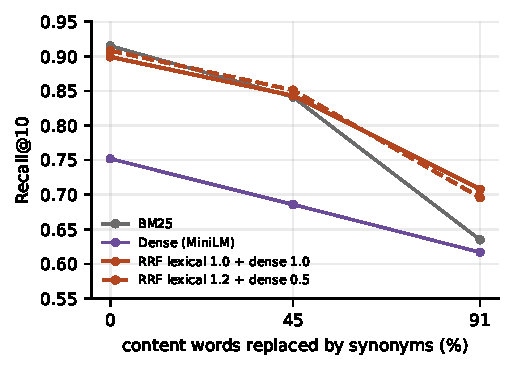
\includegraphics[width=\columnwidth]{fig_paraphrase.pdf}
\caption{Recall@10 as LoCoMo questions are rewritten with synonyms. BM25's lead is a property of literal questions; fusion overtakes it once wording drifts.}
\label{fig:para}
\end{figure}
BM25 matches stemmed surface forms only. Its lead on LoCoMo is a property of how the questions were written: annotators reused the words of the evidence. To separate the retriever from the benchmark we rewrote every question with WordNet synonyms at two strengths and scored every strategy on the original and rewritten questions against the same store (Fig.~\ref{fig:para}, Table~\ref{tab:para}). The ordering flips with the paraphrase level: fusion is one point behind BM25 on literal questions, one point ahead at 45\% replacement and seven points ahead at 91\%, and the best dense weight rises as the wording drifts. The dense route alone loses 13.5 points at full replacement against BM25's 28. The lexicon does not help, because expanding a wrong-sense synonym with its own neighbours adds noise rather than recovering the original word. WordNet first-sense substitution produces some unnatural rewrites (``paint a sunrise'' becomes ``pigment a dawn''), which is why even the dense route drops; an LLM-written paraphrase set would give a cleaner curve.

\begin{table}[t]
\caption{Recall@10 on original and paraphrased LoCoMo questions (1\,982 questions, seed 0; change in parentheses)}
\label{tab:para}
\centering
\scriptsize
\begin{tabular}{lrrr}
\toprule
System & Original & 45\% replaced & 91\% replaced \\
\midrule
BM25 & 0.915 & 0.841 ($-$7.4) & 0.635 ($-$28.0) \\
BM25 + semantic lexicon & 0.913 & 0.825 ($-$8.8) & 0.633 ($-$28.0) \\
Dense (MiniLM) & 0.752 & 0.686 ($-$6.6) & 0.617 ($-$13.5) \\
RRF lex 1.0 + dense 1.0 & 0.899 & 0.843 ($-$5.6) & \textbf{0.708} ($-$19.1) \\
RRF lex 1.2 + dense 1.0 & 0.903 & 0.843 ($-$6.0) & 0.697 ($-$20.5) \\
RRF lex 1.2 + dense 0.5 & 0.908 & \textbf{0.851} ($-$5.7) & 0.696 ($-$21.2) \\
\bottomrule
\end{tabular}
\end{table}

\subsection{The controller selects the regime from the query log}
\label{sec:regime}
\begin{figure}[t]
\centering
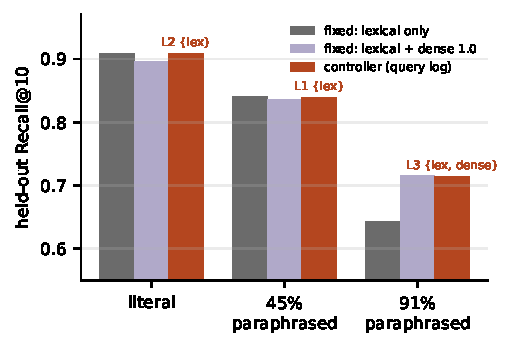
\includegraphics[width=\columnwidth]{fig_regime.pdf}
\caption{Held-out Recall@10 per query regime. The controller, calibrated on that regime's query log only, matches the best fixed configuration in each regime; neither fixed configuration does.}
\label{fig:regime}
\end{figure}
No fixed configuration is right for both regimes. We added the dense-route weight $\{0.5, 1.0\}$ to the controller's search space and ran it three times on the same store, calibrated on a 30\% calibration split of the literal, the 45\%-paraphrased and the 91\%-paraphrased questions respectively (594 probes each), scored on the other 70\% of the same regime; fixed configurations were scored on the same held-out split (Fig.~\ref{fig:regime}, Table~\ref{tab:regime}). The controller never sees the test questions. From the query log alone it switches from lexical-only to lexical+dense exactly where that switch pays, lands within 0.2--0.7 points of the best fixed configuration in every regime, and chooses a compression level under the same recall bound in the same search. Lexical-only loses seven points on paraphrased queries; lexical+dense loses one point on literal queries; the controller loses neither. In the middle regime it accepts a 0.7-point recall loss for lexical-only's lower latency: the objective minimises cost subject to retention of at least $\rho = 0.95$ of the best raw retrieval, so a gain inside the slack does not justify the dense route's cost. This is by design and should be read as such.

This is, to our knowledge, the first positive result for a query-log-adaptive sparse--dense configuration selector in agent memory. Ref.~\cite{fairness} reports an oracle headroom of 22\% over fixed blends that no lightweight adaptive router realised under cross-validation. The difference is the selector: a discrete guarded search with an out-of-sample confirmation step, rather than a per-query predictor, and a search that includes the compression level, so retrieval and storage are decided together.

\begin{table}[t]
\caption{Held-out Recall@10 per query regime; controller calibrated on that regime's query log only (seed 0)}
\label{tab:regime}
\centering
\scriptsize
\resizebox{\columnwidth}{!}{%
\begin{tabular}{llrrrr}
\toprule
Regime & Controller chose & Ctrl & Best fixed & Lex & Lex+d 1.0 \\
\midrule
Literal & L2, \{lex\} & \textbf{0.908} & 0.908 (lex) & 0.908 & 0.896 \\
45\% paraphr. & L1, \{lex\} & 0.839 & 0.846 (lex+d .5) & 0.841 & 0.836 \\
91\% paraphr. & L3, \{lex, dense\} & \textbf{0.714} & 0.716 (lex+d 1.0) & 0.643 & 0.716 \\
\bottomrule
\end{tabular}}
\end{table}

\section{LLM-Judged Answer Accuracy}
\subsection{Reader and judge on 200 LoCoMo questions ($K=5$)}
For each question a system retrieves its top-$K$ context, a Claude Opus 5.5 reader answers from that context only and abstains when it lacks the answer, and a Claude Sonnet 5.5 judge marks the answer against the gold. FidelityMem runs under its controller calibrated on the 30\% query-log split. The retrieval tie carries through to accuracy (Table~\ref{tab:llm}): FidelityMem 63.0\% against BM25 64.5\% on the same questions, inside the noise of a 200-question sample ($\pm 6.7$ points at 95\%), with equal tokens per query and equal API cost. A real architecture gap shows up as a real accuracy gap: Zep-style, 18 points lower on Recall@5, is 16.5 points lower on accuracy and abstains twice as often.

\begin{table}[t]
\caption{Answer accuracy, 200 LoCoMo session questions, $K=5$, seed 0. Categories: single-hop / multi-hop / temporal / open-domain / adversarial}
\label{tab:llm}
\centering
\scriptsize
\resizebox{\columnwidth}{!}{%
\begin{tabular}{lrrrrlr}
\toprule
System & Acc. & Abst. & R@5 & Tok/q & Categories & \$/q \\
\midrule
BM25, raw text & 64.5\% & 13.5\% & .830 & 3\,792 & .81/.38/.68/.80/.40 & .0240 \\
FM, extractive (L3, content) & 63.0\% & 14.5\% & .820 & 3\,725 & .77/.44/.70/.40/.37 & .0237 \\
FM, Claude compressor (L2, facts) & 61.5\% & 17.5\% & .814 & 2\,858 & .79/.35/.72/.80/.23 & \textbf{.0187} \\
Zep-style & 48.0\% & 30.5\% & .645 & 3\,645 & .64/.27/.47/.60/.27 & .0232 \\
\bottomrule
\end{tabular}}
\end{table}

\subsection{LLM compression at ingestion}
With the Claude compressor and extractor at ingestion (272 sessions, about 800 Opus calls, 57 minutes), gated exactly as the extractive compressor, the controller selected level 2 under the facts profile where with extractive compression it had selected level 3 under the content profile (98\% of the raw text): LLM summaries pass the fact probes while removing far more text. This is the first configuration in which compression pays on conversational data: 23\% fewer context tokens and 21\% lower reading cost per question, with accuracy 1.5 points below the extractive run and 3 below BM25, both inside the sample noise. Recall@5 is unchanged, so the accuracy difference, if real, comes from what the summaries omit rather than from retrieval. The one-off ingestion cost (about \$3.5 at list prices) is recovered after roughly 700 questions.

\subsection{Query rewriting, LLM reranking and evidence-first context}
Two LLM-side levers that published systems use to pass lexical retrieval were tested on the same questions with Claude Haiku 5.5: HyDE-style rewriting (the question expanded with the sentence a speaker would have said) and reranking a 20-candidate pool to $K=5$ (Table~\ref{tab:rerank}). Neither helps. Rewriting hurts both systems: on LoCoMo the question's own words are the best lexical key, and the hypothetical sentence adds words that match the wrong sessions. Reranking is neutral: when the gold session is in the top 20 it is already in the top 5, so a reranker has nothing to recover; the questions that fail are the ones whose evidence BM25 never surfaces at all. An evidence-first hierarchical context (retrieve 8 sessions, keep the 3 best-matching turns of each with one neighbour either side) cuts context tokens by about 30\% and cost by 20\% at unchanged Recall@5, with accuracy 63.5\% for BM25 and 58.5\% for FidelityMem, both within the sample noise of their raw-context runs. The saving is real; the accuracy gain is not.

\begin{table}[t]
\caption{Recall@5 with LLM rewriting and reranking (200 questions)}
\label{tab:rerank}
\centering
\scriptsize
\begin{tabular}{lrrrr}
\toprule
System & None & + rewrite & + rerank & + both \\
\midrule
BM25 & 0.830 & 0.818 & 0.830 & 0.808 \\
FidelityMem (controller) & 0.820 & 0.804 & 0.823 & 0.772 \\
\bottomrule
\end{tabular}
\end{table}

\section{Ablation and Negative Results}
\subsection{Ablation}
\label{sec:ablation}
\begin{figure}[t]
\centering
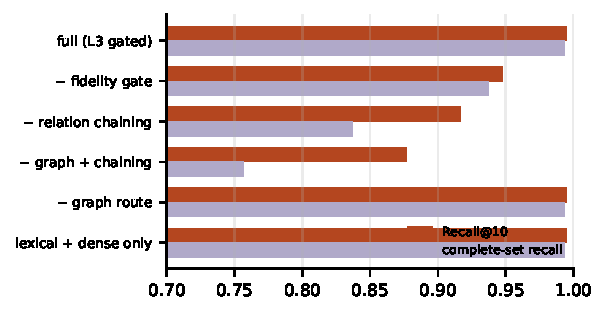
\includegraphics[width=\columnwidth]{fig_ablation.pdf}
\caption{Ablation on the synthetic benchmark ($n = 1\,000$, L3 gated, 3 seeds). Relation chaining carries the second hop; the gate carries the relation sentence through compression.}
\label{fig:ablation}
\end{figure}
One component is removed at a time from the full system (Fig.~\ref{fig:ablation}, Table~\ref{tab:ablation}). Three findings. Relation chaining is the multi-hop component: without it recall falls to 0.917 and complete-set recall to 0.837, and to 0.877 and 0.757 when the graph route is also removed; the graph route by itself mainly improves ranking (MRR 0.88 to 0.98). The gate protects relations as well as values: without it the gist drops the sentence carrying the dependency relation in 15\% of multi-hop cases, the index shrinks to the lossy-summary size, the retriever compensates with nearly three times as many raw expansions per query, and the variance across seeds triples. The content gate profile is stricter than this corpus needs: same recall, twice the storage, no expansions.

\begin{table}[t]
\caption{Ablation ($n = 1\,000$, $K=10$, level 3 gated, 3 seeds). Retain = recall relative to the full system}
\label{tab:ablation}
\centering
\scriptsize
\resizebox{\columnwidth}{!}{%
\begin{tabular}{lrrrrrr}
\toprule
Variant & R@10 & CR@10 & MRR & Tok/q & Stored & Exp./q \\
\midrule
Full (L3, gated) & 0.995 $\pm$.012 & 0.993 & 0.981 & 458 & 32\,076 & 1.11 \\
$-$ fidelity gate & 0.948 $\pm$.071 & 0.937 & 0.935 & 444 & 20\,392 & 2.97 \\
+ content gate profile & 0.995 $\pm$.012 & 0.993 & 0.929 & 762 & 73\,427 & 0.00 \\
$-$ raw expansion & 0.995 $\pm$.012 & 0.993 & 0.980 & 403 & 32\,076 & 0.00 \\
$-$ relation chaining & 0.917 $\pm$.083 & 0.837 & 0.976 & 458 & 32\,075 & 1.14 \\
$-$ graph route & 0.995 $\pm$.012 & 0.993 & 0.881 & 442 & 32\,091 & 0.86 \\
$-$ graph route and chaining & 0.877 $\pm$.019 & 0.757 & 0.881 & 440 & 32\,060 & 0.88 \\
$-$ hub penalty / pruning & 0.995 $\pm$.012 & 0.993 & 0.978 & 457 & 32\,076 & 1.10 \\
$-$ trie route & 0.995 $\pm$.012 & 0.993 & 0.978 & 458 & 32\,060 & 1.11 \\
Lexical + dense only & 0.995 $\pm$.012 & 0.993 & 0.901 & 436 & 32\,075 & 0.84 \\
\bottomrule
\end{tabular}}
\end{table}

\subsection{The semantic-codebook trie (negative result)}
\label{sec:semtrie}
A proposal raised during design: number semantically similar words with one code (a codebook from $k$-means over the embedder's word vectors), store each memory as its code sequence in a word trie so shared prefixes are stored once, and match queries in code space so synonyms hit. We built it with one safeguard, that entities, numbers, dates and negation cues are never coded, and measured storage, decode fidelity against the probes, and Recall@10 against BM25 (Table~\ref{tab:semtrie}). The storage saving exists only where text repeats (the synthetic filler) and comes from prefix sharing and stop-word dropping rather than from semantics. On real conversation the trie is larger than the raw text. The codebook does what the fidelity argument predicts: $k$-means merges neighbours, so ``machine'' decodes as ``dashboard''; the protected-token rule keeps fact-probe fidelity at 0.98 on LoCoMo, but content-word fidelity drops to 0.85 and retrieval loses 8 points to BM25. As a retrieval route at session level with 2\,000 codes it scores 0.830 alone and adds nothing to lexical + dense (Table~\ref{tab:weights}). A variant that embeds each memory as the IDF-weighted mean of its code-cluster centroids matches full dense recall on the synthetic corpus and loses 3--6 points on LoCoMo turns, for a dense index 4--9$\times$ smaller; that quantisation is the one useful outcome.

\begin{table}[t]
\caption{Semantic-codebook trie as storage}
\label{tab:semtrie}
\centering
\scriptsize
\resizebox{\columnwidth}{!}{%
\begin{tabular}{lrrrrr}
\toprule
Corpus & Bytes/raw & Fid. facts & Fid. content & R@10 trie & R@10 BM25 \\
\midrule
Synthetic, 1\,000 episodes & 0.76 & 0.81 & 0.79 & 0.875 & 0.875 \\
LoCoMo, 3 conv., 1\,451 turns & 1.08--1.10 & 0.98 & 0.85--0.87 & 0.53--0.54 & 0.613 \\
\bottomrule
\end{tabular}}
\end{table}

\subsection{The retrieval-adapted embedder and a calibration leak}
\label{sec:adapted}
Before the sentence embedder was available we trained a retrieval-adapted embedder for the dense route: pretrained word vectors with a learned weight per word (initialised from IDF) and a learned $300 \times 256$ projection (initialised to the identity), trained by InfoNCE on (question, gold evidence) pairs with in-batch and BM25 hard negatives, about a minute on CPU. On LoCoMo sessions the dense route improved from 0.287 to 0.424 and fusion from 0.726 to 0.747, still 11 points below BM25, so the controller's selection and result were unchanged (Table~\ref{tab:adapted}).

The protocol lesson matters more than the number. Our first run trained the adapter on the whole calibration split and then let the controller score route pools on the same questions, where the dense route had effectively memorised the evidence; lexical+dense looked lossless on those probes and lost ten points on the test split (controller $0.742 \pm 0.048$). Neither a tighter bound ($\rho = 0.98$) nor a recall-loss term in the cost repaired it; only disjoint data did. A learned retrieval component and a controller that selects among retrieval components must not share calibration data.

\begin{table}[t]
\caption{LoCoMo sessions, $K=5$, 3 seeds: base word vectors vs the adapted embedder (leak-free split)}
\label{tab:adapted}
\centering
\scriptsize
\begin{tabular}{lrr}
\toprule
System & Base embedder & Adapted \\
\midrule
Dense alone & 0.287 $\pm$.016 & 0.424 $\pm$.029 \\
BM25 + dense RRF & 0.726 $\pm$.005 & 0.747 $\pm$.021 \\
Zep-style & 0.687 $\pm$.023 & 0.707 $\pm$.011 \\
HippoRAG-style & 0.401 $\pm$.022 & 0.441 $\pm$.011 \\
FM raw, default routes & 0.563 $\pm$.016 & 0.610 $\pm$.016 \\
FM controller, query log & 0.849 $\pm$.014 & 0.849 $\pm$.014 \\
BM25 & 0.858 $\pm$.009 & 0.858 $\pm$.009 \\
\bottomrule
\end{tabular}
\end{table}

\section{Limitations and Threats to Validity}
\begin{enumerate}
\item \textbf{Re-implementations, not vendor code.} The six architecture baselines reproduce published retrieval designs with shared components. They are faithful to the architecture, not to the vendors' tuned systems, and a vendor system with an LLM extractor could rank differently.
\item \textbf{One real dataset.} LoCoMo at two granularities. LongMemEval has a loader and a per-question runner in the repository (controller calibrated once on held-out questions, every system rebuilt per question); its results are not in this version.
\item \textbf{Paraphrase and regime results are single-seed and WordNet-based.} First-sense synonym substitution produces unnatural rewrites, which depresses every system. Three seeds and an LLM-written paraphrase set are the obvious next step; the design of the experiment does not change.
\item \textbf{LLM evaluation is small.} 200 questions give $\pm 7$-point intervals, so the accuracy differences among BM25 and the FidelityMem variants are not significant; the Zep-style gap is.
\item \textbf{Self-probes.} The controller's self-generated probes are fact-dense sentence fragments. They suffice on fact-dense text and fail on one of three LoCoMo seeds. A deployment whose users ask about low-fact-density content needs a query log; the API accepts any probe set.
\item \textbf{Compression on chat is small at $\rho = 0.95$.} Sessions carry a fact in nearly every sentence, so the gate backs off to raw. This is the bound being enforced on text with little to remove, and is a limit of compression on this kind of text rather than of the controller. An LLM compressor under the same gate is the configuration where compression pays.
\item \textbf{Scale.} 10\,000 records in one process. The dense index is $O(n \cdot d)$ per query and the controller recompresses the store per level; beyond about $10^5$ records both need an ANN index and sampled background optimisation, which the store protocols are shaped for but which are not built. Tenant isolation is a provenance field, not an enforced partition.
\item \textbf{Retention above 1.} Compressed indexes sometimes retrieve better than raw because filler is removed; we report retention as measured and do not clip it.
\item \textbf{Construct validity of recall.} Recall@$K$ against gold episode ids measures whether the right memory is served, not whether the fact inside it survived; the fidelity gate and the LLM-judged accuracy are the two measurements that address the fact itself.
\end{enumerate}

\section{Conclusion}
A memory system can be made to keep a stated share of its evidence recall, cheaply and without labels, by generating fidelity probes from the raw source and by searching policies under that bound with an out-of-sample gate. On a controlled synthetic protocol the resulting system dominates six current memory architectures on recall and evidence completeness while halving stored and served tokens. On real conversation data it does not beat BM25, and we show why: the benchmark's questions reuse the evidence's words, and once they are paraphrased the ordering reverses. The system's value there is the controller, which selects lexical-only retrieval when the query log is literal and lexical+dense when it is paraphrased, matching the best fixed configuration in each regime without seeing the test questions, and which chooses the compression level in the same search. We also report what did not work, because a controller that can only be trusted on the configurations it was shown is the point: fixed route weights, a semantic-codebook trie, a semantic lexicon, query rewriting and LLM reranking all failed to beat the lexical baseline on this data, and a learned embedder that shared calibration data with the controller misled it. The unique parts are the gate, the controller and LLM-free ingestion; the rest is a careful integration of known components, released as an open package with the full evaluation stack.

\begin{thebibliography}{00}
\bibitem{facts} ``Facts as first-class objects: Knowledge objects for persistent LLM memory,'' arXiv:2603.17781, 2026.
\bibitem{fidelity} ``Fidelity before structure: Verbatim chunks beat lossy artifact extraction in long-conversation LLM memory,'' arXiv:2601.00821, 2026.
\bibitem{factwash} ``FACTWASH: Catching AI rewrites that wash hearsay into fact,'' arXiv:2608.03372, 2026.
\bibitem{memgpt} C. Packer et al., ``MemGPT: Towards LLMs as operating systems,'' arXiv:2310.08560, 2023.
\bibitem{hipporag} B. Guti\'errez et al., ``HippoRAG: Neurobiologically inspired long-term memory for large language models,'' arXiv:2405.14831, 2024.
\bibitem{zep} Zep / Graphiti, temporal knowledge graph memory, product documentation, 2025--2026.
\bibitem{mem0} Mem0, memory layer for AI agents, product documentation and benchmark pages, 2025--2026.
\bibitem{amem} ``A-MEM: Agentic memory for LLM agents,'' 2025.
\bibitem{r3mem} X. Wang et al., ``R$^3$Mem: Bridging memory retention and retrieval via reversible compression,'' in \emph{Findings of ACL}, 2025.
\bibitem{evolvemem} Y. Liu et al., ``EvolveMem: Self-evolving memory architecture via AutoResearch for LLM agents,'' arXiv:2605.13941, 2026.
\bibitem{memrl} Z. Zhang et al., ``MemRL: Self-evolving agents via runtime reinforcement learning on episodic memory,'' arXiv:2601.03192, 2026.
\bibitem{agentzero} ``Agent Zero Memory: Provenance-aware long-term memory for LLM agents,'' arXiv:2608.29606, 2026.
\bibitem{lazymem} ``LazyMem: Retrieve broadly, construct selectively for efficient long-term agent memory,'' arXiv:2607.22690, 2026.
\bibitem{longmemeval} D. Wu et al., ``LongMemEval: Benchmarking chat assistants on long-term interactive memory,'' arXiv:2410.10813, 2024.
\bibitem{membench} H. Tan et al., ``MemBench,'' arXiv:2506.21605, 2025.
\bibitem{dolphin} ``DolphinBench: Mapping the Pareto frontier of agent memory,'' arXiv:2609.24971, 2026.
\bibitem{crystalmem} Y. Wu and J. Huang, ``CrystalMem,'' arXiv:2608.00303, 2026.
\bibitem{arc} T. Dang et al., ``Addressable recall compaction for long context-window control in AI agents,'' arXiv:2607.25066, 2026.
\bibitem{memrefine} S. Kim et al., ``MemRefine,'' arXiv:2606.13177, 2026.
\bibitem{ratedist} A. Colaco and M. Lahjouji, ``What to keep, what to forget: A rate--distortion view of memory compaction,'' arXiv:2607.08032, 2026.
\bibitem{tfusion} ``Training-free lexical-dense fusion for conversational-memory retrieval,'' arXiv:2606.04194, 2026.
\bibitem{fairness} ``Evidence-unit fairness and the limits of query-adaptive sparse-dense fusion in financial document retrieval,'' arXiv:2608.00183, 2026.
\bibitem{wrrf} ``Optimal fusion weights form intervals, not points: A latency-aware study of query-adaptive WRRF,'' arXiv:2610.24341, 2026.
\bibitem{vstash} J. Steffens, ``vstash: Local-first hybrid retrieval with adaptive fusion for LLM agents,'' arXiv:2604.15484, 2026.
\bibitem{locomo} A. Maharana et al., ``Evaluating very long-term conversational memory of LLM agents,'' in \emph{Proc. ACL}, 2024.
\end{thebibliography}

\end{document}
